\section{Results}
\subsection{Forecast accuracy and industry heterogeneity}
Table~\ref{tab:performance} reports all forecast specifications on a common evaluation sample. Separate industry models have the lowest aggregate MAE, 3.04 pp, compared with 3.39 for the six-release mean and 3.30 for the original pooled baseline. These differences correspond to reductions of 10.3\% and 8.0\%, respectively. Elastic net (3.07), gradient boosting (3.12), and ridge (3.13) also improve on the recent-average benchmark. Partial pooling yields 3.29 pp, close to the baseline. The full unregularized dictionary yields MAE of 5.68 pp and produces six predictions outside the percentage range.

\begin{table}[!htbp]
\centering
\small
\caption{Forecast errors in percentage points. Historical: 635 forecasts at nine origins; extension: 71 forecasts at one origin; all: 706 forecasts.}\label{tab:performance}
\begin{tabular}{lrrrrr}
\toprule
Model & Historical MAE & Extension MAE & All MAE & All RMSE & All bias \\
\midrule
Persistence & 4.18 & 3.90 & 4.15 & 5.75 & -1.05 \\
Six-release mean & 3.40 & 3.34 & 3.39 & 4.64 & -2.07 \\
Baseline OLS & 3.33 & 3.09 & 3.30 & 4.55 & +0.07 \\
Linear subset & 3.39 & 3.06 & 3.36 & 4.63 & +0.03 \\
Nonlinear subset & 3.36 & 2.97 & 3.32 & 4.66 & +0.12 \\
Full OLS & 5.92 & 3.52 & 5.68 & 7.27 & +2.11 \\
Ridge & 3.15 & 2.99 & 3.13 & 4.32 & +0.47 \\
Elastic net & 3.08 & 2.93 & 3.07 & 4.29 & +0.06 \\
Gradient boosting & 3.12 & 3.09 & 3.12 & 4.38 & -0.03 \\
Partial pooling & 3.33 & 2.97 & 3.29 & 4.51 & +0.12 \\
Industry models & 3.04 & 3.02 & 3.04 & 4.29 & -0.21 \\
\bottomrule
\end{tabular}
\end{table}


Industry models beat the recent mean at nine of ten issue dates. Their mean origin-level difference is $-0.35$ pp, with exploratory block interval $[-0.46,-0.24]$. Relative to baseline OLS, the corresponding difference is $-0.26$ pp, with interval $[-0.40,-0.12]$. Ridge and boosting beat the recent mean at all ten dates. These results support industry heterogeneity and regularization within this sample, although the short evaluation history limits claims about future performance.

\begin{table}[!htbp]
\centering
\small
\caption{Paired origin-level MAE differences relative to the six-release mean. Negative values favor the fitted model. Intervals are 95\% moving-block bootstrap intervals and are exploratory.}\label{tab:paired}
\begin{tabular}{lrrr}
\toprule
Model & Difference (pp) & Interval (pp) & Origins won \\
\midrule
Baseline OLS & -0.09 & [-0.22, +0.04] & 7/10 \\
Linear subset & -0.03 & [-0.15, +0.10] & 4/10 \\
Nonlinear subset & -0.07 & [-0.20, +0.08] & 6/10 \\
Full OLS & +2.29 & [+0.71, +3.91] & 1/10 \\
Ridge & -0.25 & [-0.36, -0.17] & 10/10 \\
Elastic net & -0.32 & [-0.43, -0.21] & 9/10 \\
Gradient boosting & -0.27 & [-0.45, -0.13] & 10/10 \\
Partial pooling & -0.10 & [-0.23, +0.05] & 5/10 \\
Industry models & -0.35 & [-0.46, -0.24] & 9/10 \\
\bottomrule
\end{tabular}
\end{table}


\begin{figure}[htbp]
\centering
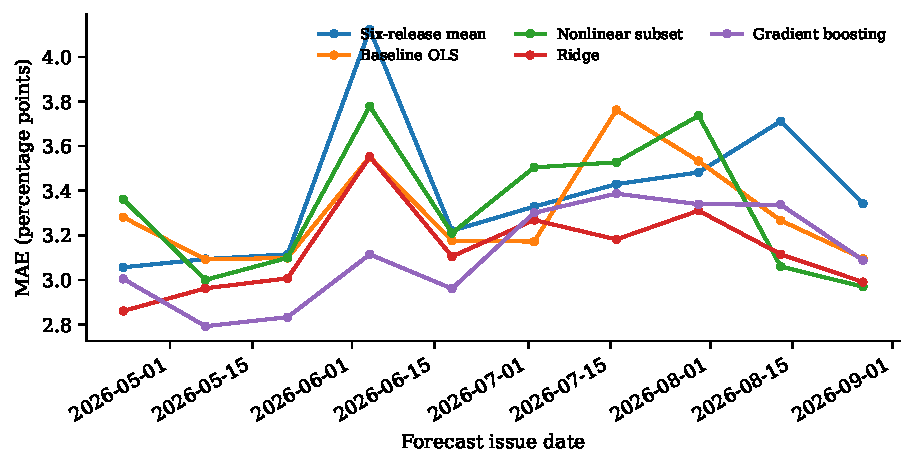
\includegraphics[width=.95\linewidth]{errors_by_origin.pdf}
\caption{Forecast MAE by issue date. All lines use identical evaluated group-release pairs. The final point forecasts the extension outcome.}
\label{fig:origins}
\end{figure}

Industry models reduce MAE for the 50--99 employee band from 5.32 pp under the baseline to 4.23 pp, below the recent mean's 4.65 pp. The advantage is not uniform: for the 10--19 employee band, ridge and elastic net perform better than separate industry models. At the industry level, Information remains difficult: its industry-model MAE is 6.48 pp. Aggregate improvement therefore does not justify equally confident forecasts for every group. The median published target standard error is 2.83 pp; 88.8\% of industry-model errors fall within twice the corresponding target standard error. This comparison describes the scale of survey uncertainty and does not establish interval calibration.

The extension contains one origin and cannot establish general superiority. Elastic net has its lowest extension MAE at 2.93 pp, followed by nonlinear subset selection at 2.97 pp. Industry models achieve 3.02 pp, compared with 3.09 for the baseline and 3.34 for the recent mean. All expanded methods remain retrospectively specified.

\subsection{Selected nonlinear structure}
The nonlinear search selects an industry-by-current-use interaction at every outer origin. Expected use squared and the current-use-by-time interaction are selected at six of ten origins; the current-by-expected-use interaction appears at the other four. Current use squared and time squared are never selected. Thus the candidate search finds industry-dependent slopes and some curvature in expectations, without evidence that a quadratic current-use response is consistently needed.

The nonlinear subset achieves aggregate MAE of 3.32 pp, compared with 3.36 for the linear subset and 3.30 for the baseline. Its mean origin-level improvement over the linear subset is only 0.03 pp, with interval $[-0.068,0.005]$ for the nonlinear-minus-linear difference. Relative to the baseline, its difference is $+0.02$ pp with interval $[-0.064,0.120]$. These comparisons provide limited support for an incremental predictive benefit from the nonlinear terms.

\begin{figure}[htbp]
\centering
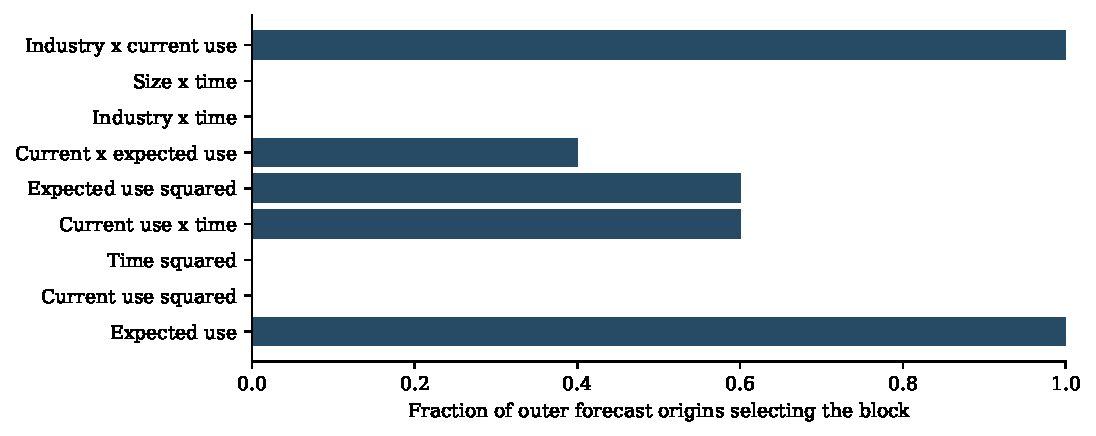
\includegraphics[width=.95\linewidth]{subset_stability.pdf}
\caption{Selection frequency of optional blocks. Main effects for current use, time, industry, and size are mandatory. An interaction with industry allows slopes to differ across sectors.}
\label{fig:selection}
\end{figure}

\begin{figure}[htbp]
\centering
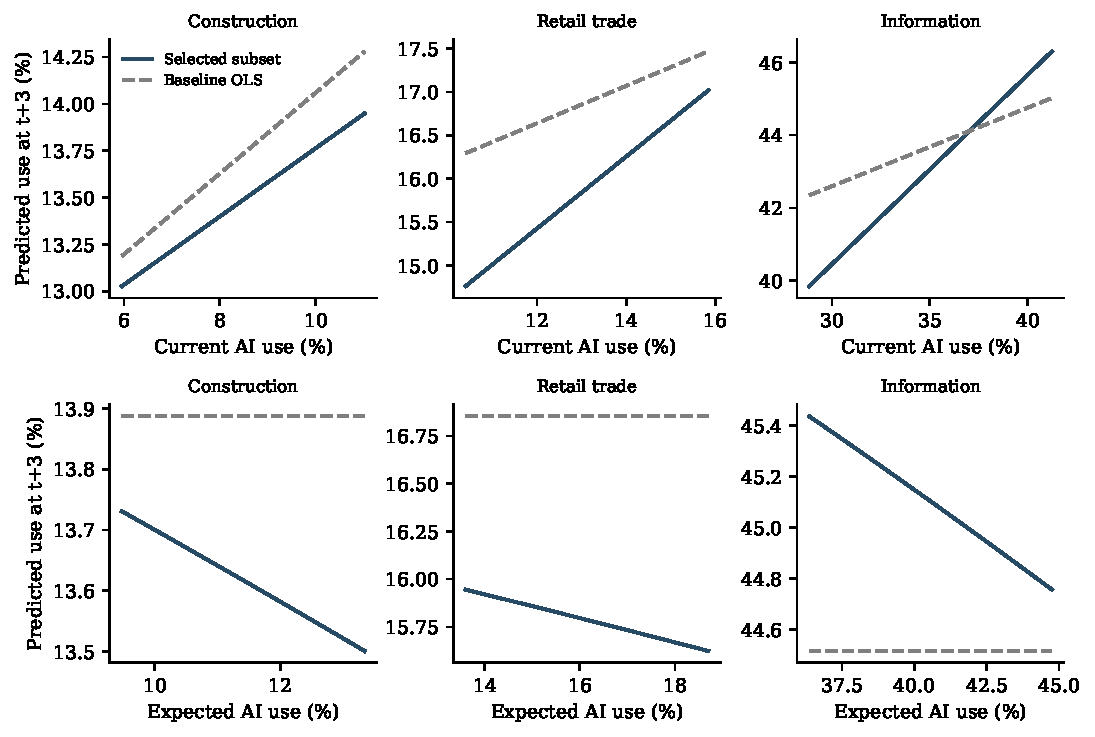
\includegraphics[width=.97\linewidth]{conditional_curves.pdf}
\caption{Conditional predictions from the final nonlinear subset and baseline, for 1--4 employee firms in three industries. The varying predictor spans its within-group training 5th--95th percentiles. The other adoption predictor is fixed at its within-group training median, and time is fixed at the final issue date. The final subset includes expected use squared; its current-use relationship is linear when time and expectations are held fixed. These curves describe fitted relationships without causal interpretation.}
\label{fig:curves}
\end{figure}

Ridge ablations reinforce the importance of recent history. Removing lagged rates, recent change, and the rolling mean increases MAE from 3.13 to 3.70 pp. Removing the six-release cycle changes MAE only to 3.15 pp. Removing quantitative curvature terms gives 3.12 pp, and omitting contemporaneous aggregate rates also gives 3.12 pp. These small latter differences do not establish useful seasonality or a material gain from the larger dictionary. The ridge search selects penalty 1,000 at all origins, even after expanding the grid to 100,000.

\subsection{Industry growth and ranking}
Finance and insurance has the highest estimated growth, 1.28 pp per four weeks, followed by Information at 1.22 and professional and technical services at 1.08. Their conditional intervals are $[1.07,1.48]$, $[0.95,1.50]$, and $[0.94,1.21]$, respectively. Accommodation and food services grows by 0.16 pp per four weeks, with interval $[0.11,0.21]$. All retained industries have positive fitted trends in the observed period. These are absolute percentage-point changes; rankings by relative percentage growth would answer a different question.

\begin{figure}[htbp]
\centering
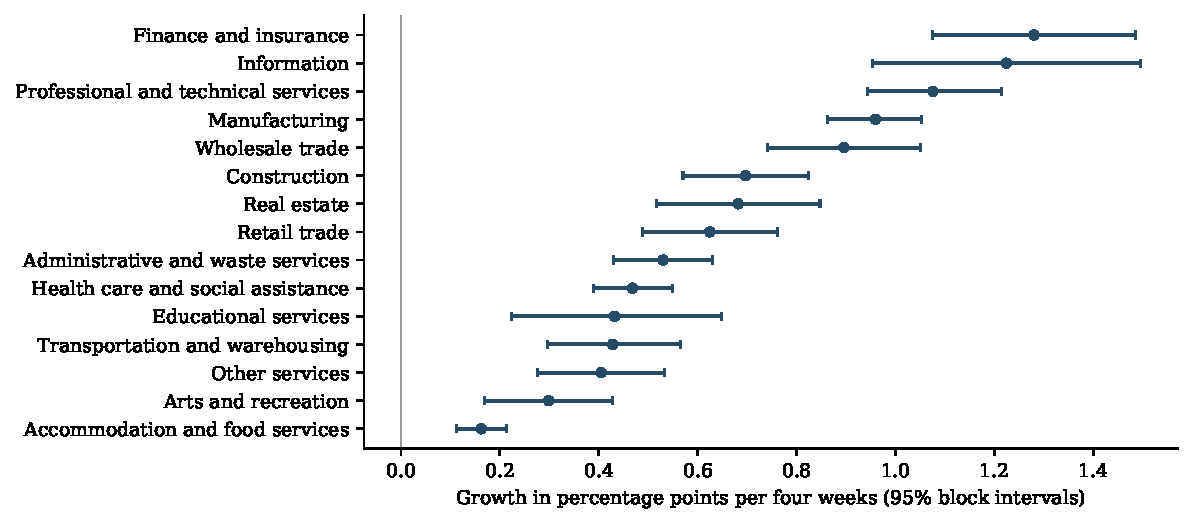
\includegraphics[width=.96\linewidth]{industry_growth.pdf}
\caption{Industry-specific growth with conditional 95\% wild block bootstrap intervals. Group intercepts account for stable industry-size differences. Results apply to retained size groups and are not population-weighted industry estimates.}
\label{fig:growth}
\end{figure}

The top two industries cannot be confidently ordered. The Information-minus-finance growth difference is $-0.06$ pp per four weeks, with interval $[-0.38,0.27]$. Finance has a bootstrap rank range of 1--3, Information 1--4, and professional services 2--3. Finance, Information, and professional services occupy the top three in 100.0\%, 97.2\%, and 97.8\% of bootstrap draws, respectively. These frequencies are conditional on the fitted trend model and a short series. They support a leading group more strongly than a precise ordering within that group.

\begin{figure}[htbp]
\centering
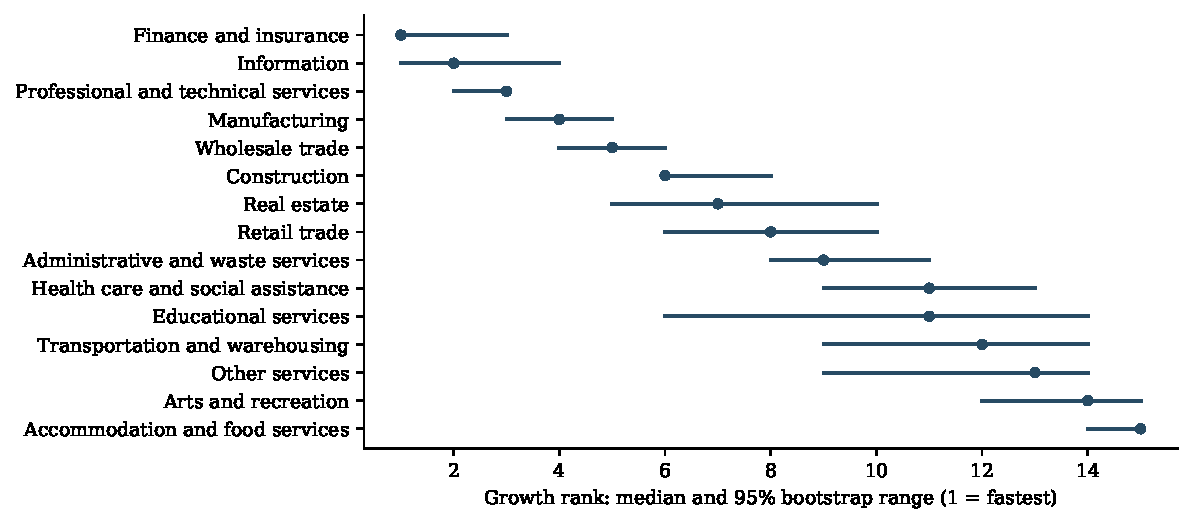
\includegraphics[width=.96\linewidth]{industry_ranks.pdf}
\caption{Median growth ranks and central 95\% bootstrap rank ranges. Overlapping ranges indicate uncertainty in exact ordering; the ranges are not simultaneous confidence sets.}
\label{fig:ranks}
\end{figure}

Adding a common sample-change indicator preserves the primary ordering closely. Inverse-variance weighting changes the relative ordering of the top two: Information's estimated growth becomes 1.16 pp per four weeks and finance's 1.14. This sensitivity is consistent with their overlapping uncertainty. The leading group remains substantively similar.

\subsection{Release chronology}
The event analysis uses 65 groups with observed rates at all 23 releases. The three earliest announcements have fewer than three pre-event reference periods in the comparable series and cannot support the specified window comparison. For the February and March events with sufficient observations, three-period pre/post changes are positive: 0.45 pp for Claude Opus 4.6, 1.43 pp for Gemini 3.1 Pro, and 1.61 pp for GPT-5.4. The reference windows overlap substantially.

\begin{figure}[htbp]
\centering
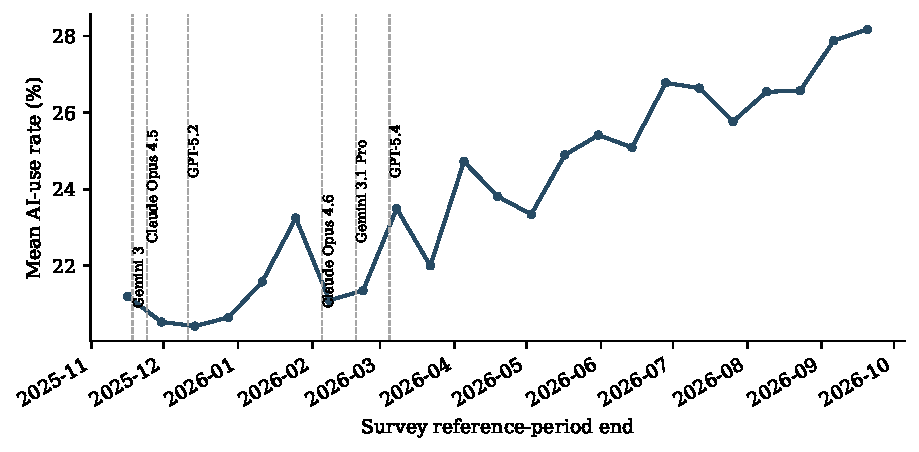
\includegraphics[width=.95\linewidth]{release_timeline.pdf}
\caption{Balanced-group AI-use mean by reference-period end, with selected provider announcement dates. Publication occurs after the reference period and collection. Event positions indicate temporal correspondence; the figure does not estimate causal effects.}
\label{fig:events}
\end{figure}

The cumulative announcement count correlates 0.81 with time. After adjustment for a linear trend and the sample-change indicator, its descriptive coefficient is $-0.47$ pp per selected announcement. This sign differs from the positive unadjusted window changes. The contrast illustrates sensitivity to trend adjustment and the limited independent information in a common event chronology. It does not establish a negative effect of model releases. The data do not separate release effects from ongoing diffusion or other calendar-time influences.

\subsection{Interpolation and overparameterization}
The random-feature design reaches full row rank, including the intercept, near $p/n=1$. Minimum-norm training error approaches zero there. Median future RMSE rises from 5.63 pp at $p/n=0.2$ to approximately 4,577 pp at interpolation. It then falls to approximately 190 pp at $p/n=1.2$, remaining near 203 pp at $p/n=2$. This post-peak reduction is a second-descent pattern over part of the tested range, but its prediction errors remain far above those of the practical forecasting models.

\begin{figure}[htbp]
\centering
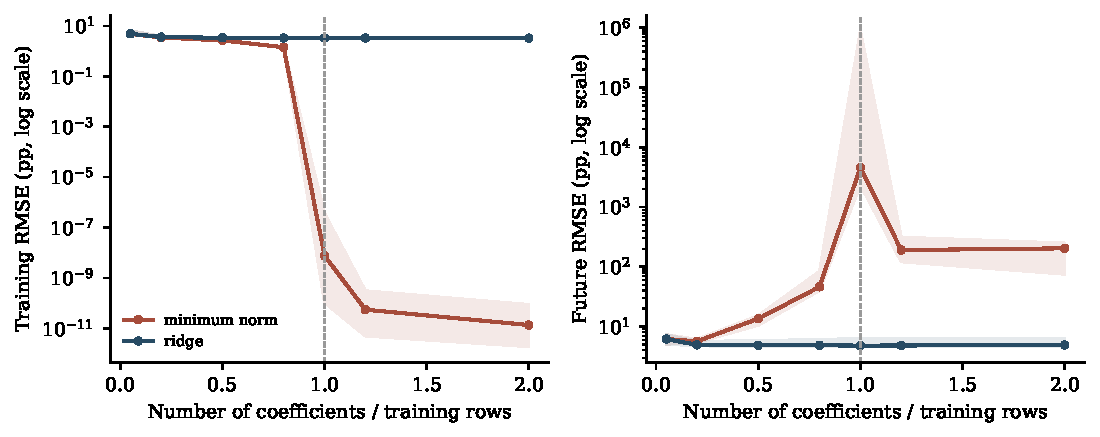
\includegraphics[width=\linewidth]{complexity.pdf}
\caption{Training and future RMSE across model widths, using logarithmic error axes. Lines show medians over three origins and three feature seeds; shading shows the 10th--90th percentiles across those nine fits, rather than confidence intervals. The vertical line marks $p/n=1$. Ridge uses a fixed diagnostic penalty of 0.01.}
\label{fig:complexity}
\end{figure}

Ridge avoids interpolation and keeps median future RMSE near 4.77--4.89 pp for $p/n$ between 1 and 2. At $p/n=2$, its median effective degrees of freedom are approximately 210, compared with a median training-row count of 912. Thus a nominally overparameterized representation can remain strongly regularized. This experiment establishes the existence of interpolating fits in the chosen representation, while providing no evidence that unregularized overparameterization improves useful forecasting performance.

The practical full OLS model already performs poorly with 81 nominal coefficients and training samples of 560--1,195 rows. Its recorded ranks are 78--80 because the dictionary includes redundant relationships. Predictive instability therefore arises well before the formal $p>n$ regime.
